\documentclass[twoside]{book}

% Packages required by doxygen
\usepackage{fixltx2e}
\usepackage{calc}
\usepackage{doxygen}
\usepackage[export]{adjustbox} % also loads graphicx
\usepackage{graphicx}
\usepackage[utf8]{inputenc}
\usepackage{makeidx}
\usepackage{multicol}
\usepackage{multirow}
\PassOptionsToPackage{warn}{textcomp}
\usepackage{textcomp}
\usepackage[nointegrals]{wasysym}
\usepackage[table]{xcolor}

% Font selection
\usepackage[T1]{fontenc}
\usepackage[scaled=.90]{helvet}
\usepackage{courier}
\usepackage{amssymb}
\usepackage{sectsty}
\renewcommand{\familydefault}{\sfdefault}
\allsectionsfont{%
  \fontseries{bc}\selectfont%
  \color{darkgray}%
}
\renewcommand{\DoxyLabelFont}{%
  \fontseries{bc}\selectfont%
  \color{darkgray}%
}
\newcommand{\+}{\discretionary{\mbox{\scriptsize$\hookleftarrow$}}{}{}}

% Page & text layout
\usepackage{geometry}
\geometry{%
  a4paper,%
  top=2.5cm,%
  bottom=2.5cm,%
  left=2.5cm,%
  right=2.5cm%
}
\tolerance=750
\hfuzz=15pt
\hbadness=750
\setlength{\emergencystretch}{15pt}
\setlength{\parindent}{0cm}
\setlength{\parskip}{0.2cm}
\makeatletter
\renewcommand{\paragraph}{%
  \@startsection{paragraph}{4}{0ex}{-1.0ex}{1.0ex}{%
    \normalfont\normalsize\bfseries\SS@parafont%
  }%
}
\renewcommand{\subparagraph}{%
  \@startsection{subparagraph}{5}{0ex}{-1.0ex}{1.0ex}{%
    \normalfont\normalsize\bfseries\SS@subparafont%
  }%
}
\makeatother

% Headers & footers
\usepackage{fancyhdr}
\pagestyle{fancyplain}
\fancyhead[LE]{\fancyplain{}{\bfseries\thepage}}
\fancyhead[CE]{\fancyplain{}{}}
\fancyhead[RE]{\fancyplain{}{\bfseries\leftmark}}
\fancyhead[LO]{\fancyplain{}{\bfseries\rightmark}}
\fancyhead[CO]{\fancyplain{}{}}
\fancyhead[RO]{\fancyplain{}{\bfseries\thepage}}
\fancyfoot[LE]{\fancyplain{}{}}
\fancyfoot[CE]{\fancyplain{}{}}
\fancyfoot[RE]{\fancyplain{}{\bfseries\scriptsize Generated on Sun May 8 2016 11\+:48\+:44 for k\+Buffer by Doxygen }}
\fancyfoot[LO]{\fancyplain{}{\bfseries\scriptsize Generated on Sun May 8 2016 11\+:48\+:44 for k\+Buffer by Doxygen }}
\fancyfoot[CO]{\fancyplain{}{}}
\fancyfoot[RO]{\fancyplain{}{}}
\renewcommand{\footrulewidth}{0.4pt}
\renewcommand{\chaptermark}[1]{%
  \markboth{#1}{}%
}
\renewcommand{\sectionmark}[1]{%
  \markright{\thesection\ #1}%
}

% Indices & bibliography
\usepackage{natbib}
\usepackage[titles]{tocloft}
\setcounter{tocdepth}{3}
\setcounter{secnumdepth}{5}
\makeindex

% Hyperlinks (required, but should be loaded last)
\usepackage{ifpdf}
\ifpdf
  \usepackage[pdftex,pagebackref=true]{hyperref}
\else
  \usepackage[ps2pdf,pagebackref=true]{hyperref}
\fi
\hypersetup{%
  colorlinks=true,%
  linkcolor=blue,%
  citecolor=blue,%
  unicode%
}

% Custom commands
\newcommand{\clearemptydoublepage}{%
  \newpage{\pagestyle{empty}\cleardoublepage}%
}


%===== C O N T E N T S =====

\begin{document}

% Titlepage & ToC
\hypersetup{pageanchor=false,
             bookmarks=true,
             bookmarksnumbered=true,
             pdfencoding=unicode
            }
\pagenumbering{roman}
\begin{titlepage}
\vspace*{7cm}
\begin{center}%
{\Large k\+Buffer \\[1ex]\large 1.\+0 }\\
\vspace*{1cm}
{\large Generated by Doxygen 1.8.9.1}\\
\vspace*{0.5cm}
{\small Sun May 8 2016 11:48:44}\\
\end{center}
\end{titlepage}
\clearemptydoublepage
\tableofcontents
\clearemptydoublepage
\pagenumbering{arabic}
\hypersetup{pageanchor=true}

%--- Begin generated contents ---
\chapter{Data Structure Index}
\section{Data Structures}
Here are the data structures with brief descriptions\+:\begin{DoxyCompactList}
\item\contentsline{section}{\hyperlink{structbuffer__t}{buffer\+\_\+t} \\*Struct for buffer handling. If you need a ringbuffer in your software, you should instantiate a \hyperlink{structbuffer__t}{buffer\+\_\+t}, and run the neccessary functions with a pointer to your instance }{\pageref{structbuffer__t}}{}
\end{DoxyCompactList}

\chapter{File Index}
\section{File List}
Here is a list of all documented files with brief descriptions\+:\begin{DoxyCompactList}
\item\contentsline{section}{k\+Buffer/\hyperlink{k_buffer_8c}{k\+Buffer.\+c} \\*A universal ringbuffer library A (more or less) universal ringbuffer library, suitable (at least) for x86 and A\+V\+R }{\pageref{k_buffer_8c}}{}
\item\contentsline{section}{k\+Buffer/\hyperlink{k_buffer_8h}{k\+Buffer.\+h} \\*A universal ringbuffer library A (more or less) universal ringbuffer library, suitable (at least) for x86 and A\+V\+R }{\pageref{k_buffer_8h}}{}
\end{DoxyCompactList}

\chapter{Data Structure Documentation}
\hypertarget{structbuffer__t}{}\section{buffer\+\_\+t Struct Reference}
\label{structbuffer__t}\index{buffer\+\_\+t@{buffer\+\_\+t}}


Struct for buffer handling. If you need a ringbuffer in your software, you should instantiate a \hyperlink{structbuffer__t}{buffer\+\_\+t}, and run the neccessary functions with a pointer to your instance.  




{\ttfamily \#include $<$k\+Buffer.\+h$>$}

\subsection*{Data Fields}
\begin{DoxyCompactItemize}
\item 
\hypertarget{structbuffer__t_a226b259859e359bec68028e844a29d13}{}uint8\+\_\+t \hyperlink{structbuffer__t_a226b259859e359bec68028e844a29d13}{is\+Initialized}\label{structbuffer__t_a226b259859e359bec68028e844a29d13}

\begin{DoxyCompactList}\small\item\em is 0 if the buffer is not initialized \end{DoxyCompactList}\item 
\hypertarget{structbuffer__t_a497ab79d85c05cf11b3042d27c5a0dbb}{}uint16\+\_\+t \hyperlink{structbuffer__t_a497ab79d85c05cf11b3042d27c5a0dbb}{write\+Pointer}\label{structbuffer__t_a497ab79d85c05cf11b3042d27c5a0dbb}

\begin{DoxyCompactList}\small\item\em The write pointer of the buffer. At a write procedure, data gets written and the pointer is incremented. \end{DoxyCompactList}\item 
\hypertarget{structbuffer__t_aae80b6cbad55ddcee74d93a23af7f88f}{}uint16\+\_\+t \hyperlink{structbuffer__t_aae80b6cbad55ddcee74d93a23af7f88f}{read\+Pointer}\label{structbuffer__t_aae80b6cbad55ddcee74d93a23af7f88f}

\begin{DoxyCompactList}\small\item\em The read pointer of the buffer. At a read procedure, data gets read and the pointer is incremented. \end{DoxyCompactList}\item 
\hypertarget{structbuffer__t_a1892eba2086d12ac2b09005aeb09ea3b}{}uint16\+\_\+t \hyperlink{structbuffer__t_a1892eba2086d12ac2b09005aeb09ea3b}{length}\label{structbuffer__t_a1892eba2086d12ac2b09005aeb09ea3b}

\begin{DoxyCompactList}\small\item\em The number of elements in the buffer. \end{DoxyCompactList}\item 
\hypertarget{structbuffer__t_ad42232a8a992b5d0eb9daf58d83337ec}{}uint8\+\_\+t \hyperlink{structbuffer__t_ad42232a8a992b5d0eb9daf58d83337ec}{element\+Length}\label{structbuffer__t_ad42232a8a992b5d0eb9daf58d83337ec}

\begin{DoxyCompactList}\small\item\em The number of bytes of one buffer element. The total memory consumption in Bytes is equal to length $\ast$ element\+Length. \end{DoxyCompactList}\item 
\hypertarget{structbuffer__t_ac7e5e46f55ed6f23cd0c8630ca768f8b}{}uint16\+\_\+t \hyperlink{structbuffer__t_ac7e5e46f55ed6f23cd0c8630ca768f8b}{datacount}\label{structbuffer__t_ac7e5e46f55ed6f23cd0c8630ca768f8b}

\begin{DoxyCompactList}\small\item\em A variable which is increased by one when new data gets written and decremented by one when data is read. \end{DoxyCompactList}\item 
\hypertarget{structbuffer__t_a974e9a505549d9f8ad9e45cb1b562413}{}buffer\+Datatype $\ast$ \hyperlink{structbuffer__t_a974e9a505549d9f8ad9e45cb1b562413}{data}\label{structbuffer__t_a974e9a505549d9f8ad9e45cb1b562413}

\begin{DoxyCompactList}\small\item\em A pointer to the first element of the buffer. Length $\ast$ element\+Length bytes of memory are allocated after this pointer. \end{DoxyCompactList}\end{DoxyCompactItemize}


\subsection{Detailed Description}
Struct for buffer handling. If you need a ringbuffer in your software, you should instantiate a \hyperlink{structbuffer__t}{buffer\+\_\+t}, and run the neccessary functions with a pointer to your instance. 

The documentation for this struct was generated from the following file\+:\begin{DoxyCompactItemize}
\item 
k\+Buffer/\hyperlink{k_buffer_8h}{k\+Buffer.\+h}\end{DoxyCompactItemize}

\chapter{File Documentation}
\hypertarget{k_buffer_8c}{}\section{k\+Buffer/k\+Buffer.c File Reference}
\label{k_buffer_8c}\index{k\+Buffer/k\+Buffer.\+c@{k\+Buffer/k\+Buffer.\+c}}


A universal ringbuffer library.  


{\ttfamily \#include \char`\"{}k\+Buffer.\+h\char`\"{}}\\*
{\ttfamily \#include $<$stdlib.\+h$>$}\\*
{\ttfamily \#include $<$math.\+h$>$}\\*
Include dependency graph for k\+Buffer.\+c\+:\nopagebreak
\begin{figure}[H]
\begin{center}
\leavevmode
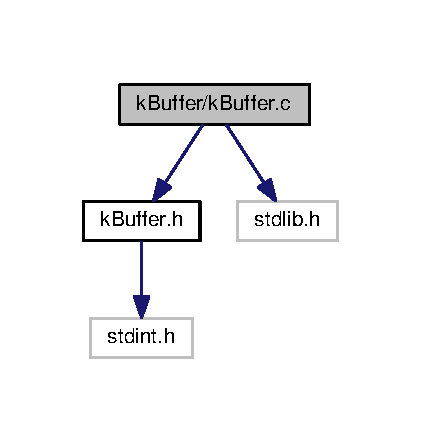
\includegraphics[width=268pt]{k_buffer_8c__incl}
\end{center}
\end{figure}
\subsection*{Functions}
\begin{DoxyCompactItemize}
\item 
\hyperlink{k_buffer_8h_a7a0bf550b7bd49d85172e409c0034fe6}{buffer\+Status\+\_\+t} \hyperlink{k_buffer_8c_aec18d6ea571b1326dbeb7ca15f4969c0}{buffer\+Init} (\hyperlink{structbuffer__t}{buffer\+\_\+t} $\ast$buffer, uint16\+\_\+t buffer\+Size)
\begin{DoxyCompactList}\small\item\em init a new buffer This function inits a new \hyperlink{structbuffer__t}{buffer\+\_\+t}.~\newline
 \end{DoxyCompactList}\item 
\hyperlink{k_buffer_8h_a7a0bf550b7bd49d85172e409c0034fe6}{buffer\+Status\+\_\+t} \hyperlink{k_buffer_8c_a8508583be1e356a243b0ce67254c516e}{buffer\+Write\+To\+Index} (\hyperlink{structbuffer__t}{buffer\+\_\+t} $\ast$buffer, uint16\+\_\+t index, \hyperlink{k_buffer_8h_ae8d6ebfbda34ebc2e00138c04b46e9b1}{buffer\+Datatype} data)
\begin{DoxyCompactList}\small\item\em write data to a specific index of the buffer. W\+A\+R\+N\+I\+N\+G\+: Take care when using this function, it is against the main concept of a ringbuffer \end{DoxyCompactList}\item 
\hyperlink{k_buffer_8h_a7a0bf550b7bd49d85172e409c0034fe6}{buffer\+Status\+\_\+t} \hyperlink{k_buffer_8c_aa0d7e2a4b6fd3da2822d7f968be74e5c}{buffer\+Read\+From\+Index} (\hyperlink{structbuffer__t}{buffer\+\_\+t} $\ast$buffer, uint16\+\_\+t index, \hyperlink{k_buffer_8h_ae8d6ebfbda34ebc2e00138c04b46e9b1}{buffer\+Datatype} $\ast$data)
\begin{DoxyCompactList}\small\item\em read data from a specifig index of the buffer W\+A\+R\+N\+I\+N\+G\+: Take care when using this function, it is against the main concept of a ringbuffer \end{DoxyCompactList}\item 
uint8\+\_\+t \hyperlink{k_buffer_8c_a5c599b9386c73ccd7b5eeb25f6cca38e}{buffer\+Is\+Empty} (\hyperlink{structbuffer__t}{buffer\+\_\+t} $\ast$buffer)
\begin{DoxyCompactList}\small\item\em Checks, wheter the buffer is empty. \end{DoxyCompactList}\item 
uint8\+\_\+t \hyperlink{k_buffer_8c_ac69b8a12a33d0cf0a5dab8feb4f7b020}{buffer\+Is\+Full} (\hyperlink{structbuffer__t}{buffer\+\_\+t} $\ast$buffer)
\begin{DoxyCompactList}\small\item\em Checks, wheter the buffer is full. \end{DoxyCompactList}\item 
\hyperlink{k_buffer_8h_a7a0bf550b7bd49d85172e409c0034fe6}{buffer\+Status\+\_\+t} \hyperlink{k_buffer_8c_a9d6410a89adf65a3ef12340ecb9bbd55}{buffer\+Write} (\hyperlink{structbuffer__t}{buffer\+\_\+t} $\ast$buffer, \hyperlink{k_buffer_8h_ae8d6ebfbda34ebc2e00138c04b46e9b1}{buffer\+Datatype} data)
\begin{DoxyCompactList}\small\item\em add data to the end of the ringbuffer \end{DoxyCompactList}\item 
\hyperlink{k_buffer_8h_a7a0bf550b7bd49d85172e409c0034fe6}{buffer\+Status\+\_\+t} \hyperlink{k_buffer_8c_a9b80be9033ccd6b5a101f811520ab4cc}{buffer\+Read} (\hyperlink{structbuffer__t}{buffer\+\_\+t} $\ast$buffer, \hyperlink{k_buffer_8h_ae8d6ebfbda34ebc2e00138c04b46e9b1}{buffer\+Datatype} $\ast$data)
\begin{DoxyCompactList}\small\item\em read data from the beginning of the buffer \end{DoxyCompactList}\item 
\hyperlink{k_buffer_8h_a7a0bf550b7bd49d85172e409c0034fe6}{buffer\+Status\+\_\+t} \hyperlink{k_buffer_8c_ac806d926fd21729feb18f8e7738e76b4}{buffer\+Fill} (\hyperlink{structbuffer__t}{buffer\+\_\+t} $\ast$buffer, \hyperlink{k_buffer_8h_ae8d6ebfbda34ebc2e00138c04b46e9b1}{buffer\+Datatype} data, uint8\+\_\+t silent)
\begin{DoxyCompactList}\small\item\em fill the whole buffer with given dummy data. \end{DoxyCompactList}\item 
\hyperlink{k_buffer_8h_a7a0bf550b7bd49d85172e409c0034fe6}{buffer\+Status\+\_\+t} \hyperlink{k_buffer_8c_afa8bb2b701cd9b7f871c12e0fabd66e1}{buffer\+Available} (\hyperlink{structbuffer__t}{buffer\+\_\+t} $\ast$buffer, uint16\+\_\+t $\ast$available)
\begin{DoxyCompactList}\small\item\em return, how many elements are stored and available in the buffer \end{DoxyCompactList}\item 
\hyperlink{k_buffer_8h_a7a0bf550b7bd49d85172e409c0034fe6}{buffer\+Status\+\_\+t} \hyperlink{k_buffer_8c_a1389f5c08210e077301c35bc3b43f681}{buffer\+Mean} (\hyperlink{structbuffer__t}{buffer\+\_\+t} $\ast$buffer, \hyperlink{k_buffer_8h_ae8d6ebfbda34ebc2e00138c04b46e9b1}{buffer\+Datatype} $\ast$mean\+Out)
\begin{DoxyCompactList}\small\item\em take the average of the whole buffer \end{DoxyCompactList}\item 
\hyperlink{k_buffer_8h_a7a0bf550b7bd49d85172e409c0034fe6}{buffer\+Status\+\_\+t} \hyperlink{k_buffer_8c_a1da694b34c0a52809c923d2d149d1348}{buffer\+Mean\+R\+M\+S} (\hyperlink{structbuffer__t}{buffer\+\_\+t} $\ast$buffer, \hyperlink{k_buffer_8h_ae8d6ebfbda34ebc2e00138c04b46e9b1}{buffer\+Datatype} $\ast$mean\+Out)
\begin{DoxyCompactList}\small\item\em take the root mean square of the whole buffer \end{DoxyCompactList}\end{DoxyCompactItemize}


\subsection{Detailed Description}
A universal ringbuffer library. 

\begin{DoxyAuthor}{Author}
Peter Kappelt 
\end{DoxyAuthor}
\begin{DoxySeeAlso}{See also}
\href{https://github.com/peterkappelt/kBuffer}{\tt https\+://github.\+com/peterkappelt/k\+Buffer} 
\end{DoxySeeAlso}
\begin{DoxyCopyright}{Copyright}
Peter Kappelt 2016; M\+I\+T License (see L\+I\+C\+E\+N\+S\+E.\+txt in the root of this repository) 
\end{DoxyCopyright}


\subsection{Function Documentation}
\hypertarget{k_buffer_8c_afa8bb2b701cd9b7f871c12e0fabd66e1}{}\index{k\+Buffer.\+c@{k\+Buffer.\+c}!buffer\+Available@{buffer\+Available}}
\index{buffer\+Available@{buffer\+Available}!k\+Buffer.\+c@{k\+Buffer.\+c}}
\subsubsection[{buffer\+Available}]{\setlength{\rightskip}{0pt plus 5cm}{\bf buffer\+Status\+\_\+t} buffer\+Available (
\begin{DoxyParamCaption}
\item[{{\bf buffer\+\_\+t} $\ast$}]{buffer, }
\item[{uint16\+\_\+t $\ast$}]{available}
\end{DoxyParamCaption}
)}\label{k_buffer_8c_afa8bb2b701cd9b7f871c12e0fabd66e1}


return, how many elements are stored and available in the buffer 


\begin{DoxyParams}{Parameters}
{\em buffer} & pointer to a \hyperlink{structbuffer__t}{buffer\+\_\+t} instance \\
\hline
{\em available} & pointer to a variable where the number of available elements should be stored \\
\hline
\end{DoxyParams}
\begin{DoxyReturn}{Returns}
an element of \hyperlink{k_buffer_8h_a7a0bf550b7bd49d85172e409c0034fe6}{buffer\+Status\+\_\+t} 
\end{DoxyReturn}

\begin{DoxyRetVals}{Return values}
{\em buffer\+O\+K} & it worked as expected \\
\hline
{\em buffer\+Not\+Initialized} & the buffer wasn\textquotesingle{}t initialized \\
\hline
\end{DoxyRetVals}
\hypertarget{k_buffer_8c_ac806d926fd21729feb18f8e7738e76b4}{}\index{k\+Buffer.\+c@{k\+Buffer.\+c}!buffer\+Fill@{buffer\+Fill}}
\index{buffer\+Fill@{buffer\+Fill}!k\+Buffer.\+c@{k\+Buffer.\+c}}
\subsubsection[{buffer\+Fill}]{\setlength{\rightskip}{0pt plus 5cm}{\bf buffer\+Status\+\_\+t} buffer\+Fill (
\begin{DoxyParamCaption}
\item[{{\bf buffer\+\_\+t} $\ast$}]{buffer, }
\item[{{\bf buffer\+Datatype}}]{data, }
\item[{uint8\+\_\+t}]{silent}
\end{DoxyParamCaption}
)}\label{k_buffer_8c_ac806d926fd21729feb18f8e7738e76b4}


fill the whole buffer with given dummy data. 


\begin{DoxyParams}{Parameters}
{\em buffer} & pointer \hyperlink{structbuffer__t}{buffer\+\_\+t} instance \\
\hline
{\em data} & data to fill the buffer with \\
\hline
{\em silent} & if this parameter is 1, the buffer will be filled with data, but the write pointer stays at its current position (usefull, if you take the mean but the buffer is not full yet. You can just prefill it, the mean will be taken with the prefilled values) \\
\hline
\end{DoxyParams}
\begin{DoxyReturn}{Returns}
an element of \hyperlink{k_buffer_8h_a7a0bf550b7bd49d85172e409c0034fe6}{buffer\+Status\+\_\+t} 
\end{DoxyReturn}

\begin{DoxyRetVals}{Return values}
{\em buffer\+O\+K} & it worked as expected \\
\hline
{\em buffer\+Not\+Initialized} & the buffer wasn\textquotesingle{}t initialized \\
\hline
\end{DoxyRetVals}
\hypertarget{k_buffer_8c_aec18d6ea571b1326dbeb7ca15f4969c0}{}\index{k\+Buffer.\+c@{k\+Buffer.\+c}!buffer\+Init@{buffer\+Init}}
\index{buffer\+Init@{buffer\+Init}!k\+Buffer.\+c@{k\+Buffer.\+c}}
\subsubsection[{buffer\+Init}]{\setlength{\rightskip}{0pt plus 5cm}{\bf buffer\+Status\+\_\+t} buffer\+Init (
\begin{DoxyParamCaption}
\item[{{\bf buffer\+\_\+t} $\ast$}]{buffer, }
\item[{uint16\+\_\+t}]{buffer\+Size}
\end{DoxyParamCaption}
)}\label{k_buffer_8c_aec18d6ea571b1326dbeb7ca15f4969c0}


init a new buffer This function inits a new \hyperlink{structbuffer__t}{buffer\+\_\+t}.~\newline
 


\begin{DoxyParams}{Parameters}
{\em buffer} & Pointer (\&) to a \hyperlink{structbuffer__t}{buffer\+\_\+t} object. \\
\hline
{\em buffer\+Size} & desired size of the buffer, the total buffer size (e.\+g. length-\/of-\/datatype $\ast$ buffer\+Size) may not exceed 2$^\wedge$16 bytes \\
\hline
\end{DoxyParams}
\begin{DoxyReturn}{Returns}
an element of \hyperlink{k_buffer_8h_a7a0bf550b7bd49d85172e409c0034fe6}{buffer\+Status\+\_\+t} 
\end{DoxyReturn}

\begin{DoxyRetVals}{Return values}
{\em buffer\+Memory\+Allocation\+Failed} & The memory allocation with malloc failed. Make sure, you have enough memory available \\
\hline
{\em buffer\+O\+K} & It seems, like everything went well \\
\hline
\end{DoxyRetVals}
\hypertarget{k_buffer_8c_a5c599b9386c73ccd7b5eeb25f6cca38e}{}\index{k\+Buffer.\+c@{k\+Buffer.\+c}!buffer\+Is\+Empty@{buffer\+Is\+Empty}}
\index{buffer\+Is\+Empty@{buffer\+Is\+Empty}!k\+Buffer.\+c@{k\+Buffer.\+c}}
\subsubsection[{buffer\+Is\+Empty}]{\setlength{\rightskip}{0pt plus 5cm}uint8\+\_\+t buffer\+Is\+Empty (
\begin{DoxyParamCaption}
\item[{{\bf buffer\+\_\+t} $\ast$}]{buffer}
\end{DoxyParamCaption}
)}\label{k_buffer_8c_a5c599b9386c73ccd7b5eeb25f6cca38e}


Checks, wheter the buffer is empty. 


\begin{DoxyParams}{Parameters}
{\em buffer} & Pointer to a \hyperlink{structbuffer__t}{buffer\+\_\+t} instance \\
\hline
\end{DoxyParams}

\begin{DoxyRetVals}{Return values}
{\em 1} & buffer is empty \\
\hline
{\em 0} & buffer is not empty \\
\hline
\end{DoxyRetVals}
\hypertarget{k_buffer_8c_ac69b8a12a33d0cf0a5dab8feb4f7b020}{}\index{k\+Buffer.\+c@{k\+Buffer.\+c}!buffer\+Is\+Full@{buffer\+Is\+Full}}
\index{buffer\+Is\+Full@{buffer\+Is\+Full}!k\+Buffer.\+c@{k\+Buffer.\+c}}
\subsubsection[{buffer\+Is\+Full}]{\setlength{\rightskip}{0pt plus 5cm}uint8\+\_\+t buffer\+Is\+Full (
\begin{DoxyParamCaption}
\item[{{\bf buffer\+\_\+t} $\ast$}]{buffer}
\end{DoxyParamCaption}
)}\label{k_buffer_8c_ac69b8a12a33d0cf0a5dab8feb4f7b020}


Checks, wheter the buffer is full. 


\begin{DoxyParams}{Parameters}
{\em buffer} & Pointer to a \hyperlink{structbuffer__t}{buffer\+\_\+t} instance \\
\hline
\end{DoxyParams}

\begin{DoxyRetVals}{Return values}
{\em 1} & buffer is full \\
\hline
{\em 0} & buffer is not full \\
\hline
\end{DoxyRetVals}
\hypertarget{k_buffer_8c_a1389f5c08210e077301c35bc3b43f681}{}\index{k\+Buffer.\+c@{k\+Buffer.\+c}!buffer\+Mean@{buffer\+Mean}}
\index{buffer\+Mean@{buffer\+Mean}!k\+Buffer.\+c@{k\+Buffer.\+c}}
\subsubsection[{buffer\+Mean}]{\setlength{\rightskip}{0pt plus 5cm}{\bf buffer\+Status\+\_\+t} buffer\+Mean (
\begin{DoxyParamCaption}
\item[{{\bf buffer\+\_\+t} $\ast$}]{buffer, }
\item[{{\bf buffer\+Datatype} $\ast$}]{mean\+Out}
\end{DoxyParamCaption}
)}\label{k_buffer_8c_a1389f5c08210e077301c35bc3b43f681}


take the average of the whole buffer 


\begin{DoxyParams}{Parameters}
{\em buffer} & pointer to a \hyperlink{structbuffer__t}{buffer\+\_\+t} instance \\
\hline
{\em mean\+Out} & pointer to a variable, where the mean will be stored \\
\hline
\end{DoxyParams}
\begin{DoxyReturn}{Returns}
a element of \hyperlink{k_buffer_8h_a7a0bf550b7bd49d85172e409c0034fe6}{buffer\+Status\+\_\+t} 
\end{DoxyReturn}

\begin{DoxyRetVals}{Return values}
{\em buffer\+O\+K} & it worked as expected, the mean is stored at the given variable \\
\hline
{\em buffer\+Not\+Initialized} & the buffer is not initialized \\
\hline
\end{DoxyRetVals}
\begin{DoxyRefDesc}{Bug}
\item[\hyperlink{bug__bug000001}{Bug}]The sum of the buffer is taken. Take precautions, that this variable won\textquotesingle{}t overflow \end{DoxyRefDesc}
\hypertarget{k_buffer_8c_a1da694b34c0a52809c923d2d149d1348}{}\index{k\+Buffer.\+c@{k\+Buffer.\+c}!buffer\+Mean\+R\+M\+S@{buffer\+Mean\+R\+M\+S}}
\index{buffer\+Mean\+R\+M\+S@{buffer\+Mean\+R\+M\+S}!k\+Buffer.\+c@{k\+Buffer.\+c}}
\subsubsection[{buffer\+Mean\+R\+M\+S}]{\setlength{\rightskip}{0pt plus 5cm}{\bf buffer\+Status\+\_\+t} buffer\+Mean\+R\+M\+S (
\begin{DoxyParamCaption}
\item[{{\bf buffer\+\_\+t} $\ast$}]{buffer, }
\item[{{\bf buffer\+Datatype} $\ast$}]{mean\+Out}
\end{DoxyParamCaption}
)}\label{k_buffer_8c_a1da694b34c0a52809c923d2d149d1348}


take the root mean square of the whole buffer 


\begin{DoxyParams}{Parameters}
{\em buffer} & pointer to a \hyperlink{structbuffer__t}{buffer\+\_\+t} instance \\
\hline
{\em mean\+Out} & pointer to a variable, where the mean will be stored \\
\hline
\end{DoxyParams}
\begin{DoxyReturn}{Returns}
a element of \hyperlink{k_buffer_8h_a7a0bf550b7bd49d85172e409c0034fe6}{buffer\+Status\+\_\+t} 
\end{DoxyReturn}

\begin{DoxyRetVals}{Return values}
{\em buffer\+O\+K} & it worked as expected, the mean is stored at the given variable \\
\hline
{\em buffer\+Not\+Initialized} & the buffer is not initialized \\
\hline
\end{DoxyRetVals}
\begin{DoxyRefDesc}{Bug}
\item[\hyperlink{bug__bug000002}{Bug}]The sum of squared buffer elements is taken. Take precautions, that this variable won\textquotesingle{}t overflow \end{DoxyRefDesc}
\hypertarget{k_buffer_8c_a9b80be9033ccd6b5a101f811520ab4cc}{}\index{k\+Buffer.\+c@{k\+Buffer.\+c}!buffer\+Read@{buffer\+Read}}
\index{buffer\+Read@{buffer\+Read}!k\+Buffer.\+c@{k\+Buffer.\+c}}
\subsubsection[{buffer\+Read}]{\setlength{\rightskip}{0pt plus 5cm}{\bf buffer\+Status\+\_\+t} buffer\+Read (
\begin{DoxyParamCaption}
\item[{{\bf buffer\+\_\+t} $\ast$}]{buffer, }
\item[{{\bf buffer\+Datatype} $\ast$}]{data}
\end{DoxyParamCaption}
)}\label{k_buffer_8c_a9b80be9033ccd6b5a101f811520ab4cc}


read data from the beginning of the buffer 


\begin{DoxyParams}{Parameters}
{\em buffer} & pointer to a \hyperlink{structbuffer__t}{buffer\+\_\+t} instance \\
\hline
{\em data} & pointer to a variable where data should be stored \\
\hline
\end{DoxyParams}
\begin{DoxyReturn}{Returns}
a element of \hyperlink{k_buffer_8h_a7a0bf550b7bd49d85172e409c0034fe6}{buffer\+Status\+\_\+t} 
\end{DoxyReturn}

\begin{DoxyRetVals}{Return values}
{\em buffer\+O\+K} & it worked as expected \\
\hline
{\em buffer\+Not\+Initialized} & the \hyperlink{k_buffer_8c_aec18d6ea571b1326dbeb7ca15f4969c0}{buffer\+Init()} method hasn\textquotesingle{}t been called or failed before \\
\hline
{\em buffer\+Empty} & the buffer is empty an no more data can be read \\
\hline
\end{DoxyRetVals}
\hypertarget{k_buffer_8c_aa0d7e2a4b6fd3da2822d7f968be74e5c}{}\index{k\+Buffer.\+c@{k\+Buffer.\+c}!buffer\+Read\+From\+Index@{buffer\+Read\+From\+Index}}
\index{buffer\+Read\+From\+Index@{buffer\+Read\+From\+Index}!k\+Buffer.\+c@{k\+Buffer.\+c}}
\subsubsection[{buffer\+Read\+From\+Index}]{\setlength{\rightskip}{0pt plus 5cm}{\bf buffer\+Status\+\_\+t} buffer\+Read\+From\+Index (
\begin{DoxyParamCaption}
\item[{{\bf buffer\+\_\+t} $\ast$}]{buffer, }
\item[{uint16\+\_\+t}]{index, }
\item[{{\bf buffer\+Datatype} $\ast$}]{data}
\end{DoxyParamCaption}
)}\label{k_buffer_8c_aa0d7e2a4b6fd3da2822d7f968be74e5c}


read data from a specifig index of the buffer W\+A\+R\+N\+I\+N\+G\+: Take care when using this function, it is against the main concept of a ringbuffer 


\begin{DoxyParams}{Parameters}
{\em buffer} & Pointer to a \hyperlink{structbuffer__t}{buffer\+\_\+t} instance \\
\hline
{\em index} & The index, where data should be written.~\newline
It can be in range 0 to length -\/ 1 \\
\hline
{\em data} & Pointer to a variable where the read data should be written to. \\
\hline
\end{DoxyParams}
\begin{DoxyReturn}{Returns}
an element of \hyperlink{k_buffer_8h_a7a0bf550b7bd49d85172e409c0034fe6}{buffer\+Status\+\_\+t} 
\end{DoxyReturn}

\begin{DoxyRetVals}{Return values}
{\em buffer\+O\+K} & It went successfull \\
\hline
{\em buffer\+Not\+Initialized} & The buffer is not initialized. You have to call buffer\+Init before (or the init failed before) \\
\hline
{\em buffer\+Error} & The desired data index is out of range \\
\hline
\end{DoxyRetVals}
\hypertarget{k_buffer_8c_a9d6410a89adf65a3ef12340ecb9bbd55}{}\index{k\+Buffer.\+c@{k\+Buffer.\+c}!buffer\+Write@{buffer\+Write}}
\index{buffer\+Write@{buffer\+Write}!k\+Buffer.\+c@{k\+Buffer.\+c}}
\subsubsection[{buffer\+Write}]{\setlength{\rightskip}{0pt plus 5cm}{\bf buffer\+Status\+\_\+t} buffer\+Write (
\begin{DoxyParamCaption}
\item[{{\bf buffer\+\_\+t} $\ast$}]{buffer, }
\item[{{\bf buffer\+Datatype}}]{data}
\end{DoxyParamCaption}
)}\label{k_buffer_8c_a9d6410a89adf65a3ef12340ecb9bbd55}


add data to the end of the ringbuffer 


\begin{DoxyParams}{Parameters}
{\em buffer} & pointer to a \hyperlink{structbuffer__t}{buffer\+\_\+t} instance \\
\hline
{\em data} & data which should be written \\
\hline
\end{DoxyParams}
\begin{DoxyReturn}{Returns}
a element of \hyperlink{k_buffer_8h_a7a0bf550b7bd49d85172e409c0034fe6}{buffer\+Status\+\_\+t} 
\end{DoxyReturn}

\begin{DoxyRetVals}{Return values}
{\em buffer\+O\+K} & it worked as expected \\
\hline
{\em buffer\+Not\+Initialized} & the \hyperlink{k_buffer_8c_aec18d6ea571b1326dbeb7ca15f4969c0}{buffer\+Init()} method hasn\textquotesingle{}t been called or failed before \\
\hline
{\em buffer\+Full} & the buffer is full an no more data can be written \\
\hline
\end{DoxyRetVals}
\hypertarget{k_buffer_8c_a8508583be1e356a243b0ce67254c516e}{}\index{k\+Buffer.\+c@{k\+Buffer.\+c}!buffer\+Write\+To\+Index@{buffer\+Write\+To\+Index}}
\index{buffer\+Write\+To\+Index@{buffer\+Write\+To\+Index}!k\+Buffer.\+c@{k\+Buffer.\+c}}
\subsubsection[{buffer\+Write\+To\+Index}]{\setlength{\rightskip}{0pt plus 5cm}{\bf buffer\+Status\+\_\+t} buffer\+Write\+To\+Index (
\begin{DoxyParamCaption}
\item[{{\bf buffer\+\_\+t} $\ast$}]{buffer, }
\item[{uint16\+\_\+t}]{index, }
\item[{{\bf buffer\+Datatype}}]{data}
\end{DoxyParamCaption}
)}\label{k_buffer_8c_a8508583be1e356a243b0ce67254c516e}


write data to a specific index of the buffer. W\+A\+R\+N\+I\+N\+G\+: Take care when using this function, it is against the main concept of a ringbuffer 


\begin{DoxyParams}{Parameters}
{\em buffer} & Pointer to a \hyperlink{structbuffer__t}{buffer\+\_\+t} instance \\
\hline
{\em index} & The index, where data should be written.~\newline
It can be in range 0 to length -\/ 1 \\
\hline
{\em data} & The actual data which should be written \\
\hline
\end{DoxyParams}
\begin{DoxyReturn}{Returns}
an element of \hyperlink{k_buffer_8h_a7a0bf550b7bd49d85172e409c0034fe6}{buffer\+Status\+\_\+t} 
\end{DoxyReturn}

\begin{DoxyRetVals}{Return values}
{\em buffer\+O\+K} & It went successfull \\
\hline
{\em buffer\+Not\+Initialized} & The buffer is not initialized. You have to call buffer\+Init before (or the init failed before) \\
\hline
{\em buffer\+Error} & The desired data index is out of range \\
\hline
\end{DoxyRetVals}

\hypertarget{k_buffer_8h}{}\section{k\+Buffer/k\+Buffer.h File Reference}
\label{k_buffer_8h}\index{k\+Buffer/k\+Buffer.\+h@{k\+Buffer/k\+Buffer.\+h}}


A universal ringbuffer library.  


{\ttfamily \#include $<$stdint.\+h$>$}\\*
Include dependency graph for k\+Buffer.\+h\+:\nopagebreak
\begin{figure}[H]
\begin{center}
\leavevmode
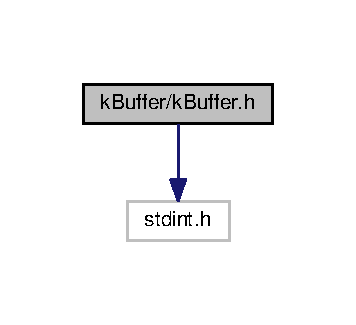
\includegraphics[width=171pt]{k_buffer_8h__incl}
\end{center}
\end{figure}
This graph shows which files directly or indirectly include this file\+:\nopagebreak
\begin{figure}[H]
\begin{center}
\leavevmode
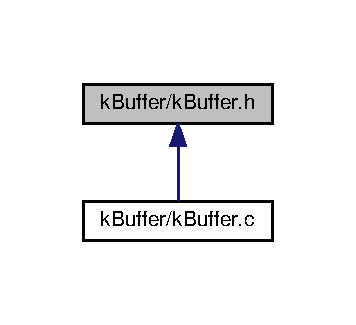
\includegraphics[width=171pt]{k_buffer_8h__dep__incl}
\end{center}
\end{figure}
\subsection*{Data Structures}
\begin{DoxyCompactItemize}
\item 
struct \hyperlink{structbuffer__t}{buffer\+\_\+t}
\begin{DoxyCompactList}\small\item\em Struct for buffer handling. If you need a ringbuffer in your software, you should instantiate a \hyperlink{structbuffer__t}{buffer\+\_\+t}, and run the neccessary functions with a pointer to your instance. \end{DoxyCompactList}\end{DoxyCompactItemize}
\subsection*{Macros}
\begin{DoxyCompactItemize}
\item 
\hypertarget{k_buffer_8h_ae8d6ebfbda34ebc2e00138c04b46e9b1}{}\#define \hyperlink{k_buffer_8h_ae8d6ebfbda34ebc2e00138c04b46e9b1}{buffer\+Datatype}~uint16\+\_\+t\label{k_buffer_8h_ae8d6ebfbda34ebc2e00138c04b46e9b1}

\begin{DoxyCompactList}\small\item\em The datatype of one buffer element. As default, it is an 16 bit unsigned integer. Feel free to change it to your needs. \end{DoxyCompactList}\end{DoxyCompactItemize}
\subsection*{Enumerations}
\begin{DoxyCompactItemize}
\item 
enum \hyperlink{k_buffer_8h_a7a0bf550b7bd49d85172e409c0034fe6}{buffer\+Status\+\_\+t} \{ \\*
\hyperlink{k_buffer_8h_a7a0bf550b7bd49d85172e409c0034fe6a69e32851bd2f089b06555decd80aac1b}{buffer\+O\+K} = 0, 
\hyperlink{k_buffer_8h_a7a0bf550b7bd49d85172e409c0034fe6a6cca9e2a7ecf10052a07be6c0eb252b5}{buffer\+Memory\+Allocation\+Failed}, 
\hyperlink{k_buffer_8h_a7a0bf550b7bd49d85172e409c0034fe6a5f17467af6ed92f0d7888dcb7feb4002}{buffer\+Empty}, 
\hyperlink{k_buffer_8h_a7a0bf550b7bd49d85172e409c0034fe6ada11f0b96f4a2a828b511c9f713eaeba}{buffer\+Full}, 
\\*
\hyperlink{k_buffer_8h_a7a0bf550b7bd49d85172e409c0034fe6a4443de2adc482ee2e06cedc60cd5a299}{buffer\+Not\+Initialized}, 
\hyperlink{k_buffer_8h_a7a0bf550b7bd49d85172e409c0034fe6a0620283513c857f87186899770dd2c2e}{buffer\+Error}
 \}
\begin{DoxyCompactList}\small\item\em buffer function return codes \end{DoxyCompactList}\end{DoxyCompactItemize}
\subsection*{Functions}
\begin{DoxyCompactItemize}
\item 
\hyperlink{k_buffer_8h_a7a0bf550b7bd49d85172e409c0034fe6}{buffer\+Status\+\_\+t} \hyperlink{k_buffer_8h_aec18d6ea571b1326dbeb7ca15f4969c0}{buffer\+Init} (\hyperlink{structbuffer__t}{buffer\+\_\+t} $\ast$buffer, uint16\+\_\+t buffer\+Size)
\begin{DoxyCompactList}\small\item\em init a new buffer This function inits a new \hyperlink{structbuffer__t}{buffer\+\_\+t}.~\newline
 \end{DoxyCompactList}\item 
\hyperlink{k_buffer_8h_a7a0bf550b7bd49d85172e409c0034fe6}{buffer\+Status\+\_\+t} \hyperlink{k_buffer_8h_a8508583be1e356a243b0ce67254c516e}{buffer\+Write\+To\+Index} (\hyperlink{structbuffer__t}{buffer\+\_\+t} $\ast$buffer, uint16\+\_\+t index, \hyperlink{k_buffer_8h_ae8d6ebfbda34ebc2e00138c04b46e9b1}{buffer\+Datatype} data)
\begin{DoxyCompactList}\small\item\em write data to a specific index of the buffer. W\+A\+R\+N\+I\+N\+G\+: Take care when using this function, it is against the main concept of a ringbuffer \end{DoxyCompactList}\item 
\hyperlink{k_buffer_8h_a7a0bf550b7bd49d85172e409c0034fe6}{buffer\+Status\+\_\+t} \hyperlink{k_buffer_8h_aa0d7e2a4b6fd3da2822d7f968be74e5c}{buffer\+Read\+From\+Index} (\hyperlink{structbuffer__t}{buffer\+\_\+t} $\ast$buffer, uint16\+\_\+t index, \hyperlink{k_buffer_8h_ae8d6ebfbda34ebc2e00138c04b46e9b1}{buffer\+Datatype} $\ast$data)
\begin{DoxyCompactList}\small\item\em read data from a specifig index of the buffer W\+A\+R\+N\+I\+N\+G\+: Take care when using this function, it is against the main concept of a ringbuffer \end{DoxyCompactList}\item 
uint8\+\_\+t \hyperlink{k_buffer_8h_a5c599b9386c73ccd7b5eeb25f6cca38e}{buffer\+Is\+Empty} (\hyperlink{structbuffer__t}{buffer\+\_\+t} $\ast$buffer)
\begin{DoxyCompactList}\small\item\em Checks, wheter the buffer is empty. \end{DoxyCompactList}\item 
uint8\+\_\+t \hyperlink{k_buffer_8h_ac69b8a12a33d0cf0a5dab8feb4f7b020}{buffer\+Is\+Full} (\hyperlink{structbuffer__t}{buffer\+\_\+t} $\ast$buffer)
\begin{DoxyCompactList}\small\item\em Checks, wheter the buffer is full. \end{DoxyCompactList}\item 
\hyperlink{k_buffer_8h_a7a0bf550b7bd49d85172e409c0034fe6}{buffer\+Status\+\_\+t} \hyperlink{k_buffer_8h_a9d6410a89adf65a3ef12340ecb9bbd55}{buffer\+Write} (\hyperlink{structbuffer__t}{buffer\+\_\+t} $\ast$buffer, \hyperlink{k_buffer_8h_ae8d6ebfbda34ebc2e00138c04b46e9b1}{buffer\+Datatype} data)
\begin{DoxyCompactList}\small\item\em add data to the end of the ringbuffer \end{DoxyCompactList}\item 
\hyperlink{k_buffer_8h_a7a0bf550b7bd49d85172e409c0034fe6}{buffer\+Status\+\_\+t} \hyperlink{k_buffer_8h_a9b80be9033ccd6b5a101f811520ab4cc}{buffer\+Read} (\hyperlink{structbuffer__t}{buffer\+\_\+t} $\ast$buffer, \hyperlink{k_buffer_8h_ae8d6ebfbda34ebc2e00138c04b46e9b1}{buffer\+Datatype} $\ast$data)
\begin{DoxyCompactList}\small\item\em read data from the beginning of the buffer \end{DoxyCompactList}\end{DoxyCompactItemize}


\subsection{Detailed Description}
A universal ringbuffer library. 

\begin{DoxyAuthor}{Author}
Peter Kappelt 
\end{DoxyAuthor}
\begin{DoxySeeAlso}{See also}
\href{https://github.com/peterkappelt/kBuffer}{\tt https\+://github.\+com/peterkappelt/k\+Buffer} 
\end{DoxySeeAlso}
\begin{DoxyCopyright}{Copyright}
Peter Kappelt 2016; M\+I\+T License (see L\+I\+C\+E\+N\+S\+E.\+txt in the root of this repository) 
\end{DoxyCopyright}


\subsection{Enumeration Type Documentation}
\hypertarget{k_buffer_8h_a7a0bf550b7bd49d85172e409c0034fe6}{}\index{k\+Buffer.\+h@{k\+Buffer.\+h}!buffer\+Status\+\_\+t@{buffer\+Status\+\_\+t}}
\index{buffer\+Status\+\_\+t@{buffer\+Status\+\_\+t}!k\+Buffer.\+h@{k\+Buffer.\+h}}
\subsubsection[{buffer\+Status\+\_\+t}]{\setlength{\rightskip}{0pt plus 5cm}enum {\bf buffer\+Status\+\_\+t}}\label{k_buffer_8h_a7a0bf550b7bd49d85172e409c0034fe6}


buffer function return codes 

\begin{Desc}
\item[Enumerator]\par
\begin{description}
\index{buffer\+O\+K@{buffer\+O\+K}!k\+Buffer.\+h@{k\+Buffer.\+h}}\index{k\+Buffer.\+h@{k\+Buffer.\+h}!buffer\+O\+K@{buffer\+O\+K}}\item[{\em 
\hypertarget{k_buffer_8h_a7a0bf550b7bd49d85172e409c0034fe6a69e32851bd2f089b06555decd80aac1b}{}buffer\+O\+K\label{k_buffer_8h_a7a0bf550b7bd49d85172e409c0034fe6a69e32851bd2f089b06555decd80aac1b}
}]it seems, as everything worked as expected \index{buffer\+Memory\+Allocation\+Failed@{buffer\+Memory\+Allocation\+Failed}!k\+Buffer.\+h@{k\+Buffer.\+h}}\index{k\+Buffer.\+h@{k\+Buffer.\+h}!buffer\+Memory\+Allocation\+Failed@{buffer\+Memory\+Allocation\+Failed}}\item[{\em 
\hypertarget{k_buffer_8h_a7a0bf550b7bd49d85172e409c0034fe6a6cca9e2a7ecf10052a07be6c0eb252b5}{}buffer\+Memory\+Allocation\+Failed\label{k_buffer_8h_a7a0bf550b7bd49d85172e409c0034fe6a6cca9e2a7ecf10052a07be6c0eb252b5}
}]happens while allocating memory,~\newline
there is not enough free memory (-\/$>$malloc failed) \index{buffer\+Empty@{buffer\+Empty}!k\+Buffer.\+h@{k\+Buffer.\+h}}\index{k\+Buffer.\+h@{k\+Buffer.\+h}!buffer\+Empty@{buffer\+Empty}}\item[{\em 
\hypertarget{k_buffer_8h_a7a0bf550b7bd49d85172e409c0034fe6a5f17467af6ed92f0d7888dcb7feb4002}{}buffer\+Empty\label{k_buffer_8h_a7a0bf550b7bd49d85172e409c0034fe6a5f17467af6ed92f0d7888dcb7feb4002}
}]happens at reading data,~\newline
buffer is empty and there is no more data to read \index{buffer\+Full@{buffer\+Full}!k\+Buffer.\+h@{k\+Buffer.\+h}}\index{k\+Buffer.\+h@{k\+Buffer.\+h}!buffer\+Full@{buffer\+Full}}\item[{\em 
\hypertarget{k_buffer_8h_a7a0bf550b7bd49d85172e409c0034fe6ada11f0b96f4a2a828b511c9f713eaeba}{}buffer\+Full\label{k_buffer_8h_a7a0bf550b7bd49d85172e409c0034fe6ada11f0b96f4a2a828b511c9f713eaeba}
}]happens at writing data,~\newline
buffer is full, no more data can be written \index{buffer\+Not\+Initialized@{buffer\+Not\+Initialized}!k\+Buffer.\+h@{k\+Buffer.\+h}}\index{k\+Buffer.\+h@{k\+Buffer.\+h}!buffer\+Not\+Initialized@{buffer\+Not\+Initialized}}\item[{\em 
\hypertarget{k_buffer_8h_a7a0bf550b7bd49d85172e409c0034fe6a4443de2adc482ee2e06cedc60cd5a299}{}buffer\+Not\+Initialized\label{k_buffer_8h_a7a0bf550b7bd49d85172e409c0034fe6a4443de2adc482ee2e06cedc60cd5a299}
}]The buffer is not initialized \index{buffer\+Error@{buffer\+Error}!k\+Buffer.\+h@{k\+Buffer.\+h}}\index{k\+Buffer.\+h@{k\+Buffer.\+h}!buffer\+Error@{buffer\+Error}}\item[{\em 
\hypertarget{k_buffer_8h_a7a0bf550b7bd49d85172e409c0034fe6a0620283513c857f87186899770dd2c2e}{}buffer\+Error\label{k_buffer_8h_a7a0bf550b7bd49d85172e409c0034fe6a0620283513c857f87186899770dd2c2e}
}]an error occured, which isn\textquotesingle{}t explained nearer. Have a look at the according function \end{description}
\end{Desc}


\subsection{Function Documentation}
\hypertarget{k_buffer_8h_aec18d6ea571b1326dbeb7ca15f4969c0}{}\index{k\+Buffer.\+h@{k\+Buffer.\+h}!buffer\+Init@{buffer\+Init}}
\index{buffer\+Init@{buffer\+Init}!k\+Buffer.\+h@{k\+Buffer.\+h}}
\subsubsection[{buffer\+Init}]{\setlength{\rightskip}{0pt plus 5cm}{\bf buffer\+Status\+\_\+t} buffer\+Init (
\begin{DoxyParamCaption}
\item[{{\bf buffer\+\_\+t} $\ast$}]{buffer, }
\item[{uint16\+\_\+t}]{buffer\+Size}
\end{DoxyParamCaption}
)}\label{k_buffer_8h_aec18d6ea571b1326dbeb7ca15f4969c0}


init a new buffer This function inits a new \hyperlink{structbuffer__t}{buffer\+\_\+t}.~\newline
 


\begin{DoxyParams}{Parameters}
{\em buffer} & Pointer (\&) to a \hyperlink{structbuffer__t}{buffer\+\_\+t} object. \\
\hline
{\em buffer\+Size} & desired size of the buffer, the total buffer size (e.\+g. length-\/of-\/datatype $\ast$ buffer\+Size) may not exceed 2$^\wedge$16 bytes \\
\hline
\end{DoxyParams}
\begin{DoxyReturn}{Returns}
an element of \hyperlink{k_buffer_8h_a7a0bf550b7bd49d85172e409c0034fe6}{buffer\+Status\+\_\+t} 
\end{DoxyReturn}

\begin{DoxyRetVals}{Return values}
{\em buffer\+Memory\+Allocation\+Failed} & The memory allocation with malloc failed. Make sure, you have enough memory available \\
\hline
{\em buffer\+O\+K} & It seems, like everything went well \\
\hline
\end{DoxyRetVals}
\hypertarget{k_buffer_8h_a5c599b9386c73ccd7b5eeb25f6cca38e}{}\index{k\+Buffer.\+h@{k\+Buffer.\+h}!buffer\+Is\+Empty@{buffer\+Is\+Empty}}
\index{buffer\+Is\+Empty@{buffer\+Is\+Empty}!k\+Buffer.\+h@{k\+Buffer.\+h}}
\subsubsection[{buffer\+Is\+Empty}]{\setlength{\rightskip}{0pt plus 5cm}uint8\+\_\+t buffer\+Is\+Empty (
\begin{DoxyParamCaption}
\item[{{\bf buffer\+\_\+t} $\ast$}]{buffer}
\end{DoxyParamCaption}
)}\label{k_buffer_8h_a5c599b9386c73ccd7b5eeb25f6cca38e}


Checks, wheter the buffer is empty. 


\begin{DoxyParams}{Parameters}
{\em buffer} & Pointer to a \hyperlink{structbuffer__t}{buffer\+\_\+t} instance \\
\hline
\end{DoxyParams}

\begin{DoxyRetVals}{Return values}
{\em 1} & buffer is empty \\
\hline
{\em 0} & buffer is not empty \\
\hline
\end{DoxyRetVals}
\hypertarget{k_buffer_8h_ac69b8a12a33d0cf0a5dab8feb4f7b020}{}\index{k\+Buffer.\+h@{k\+Buffer.\+h}!buffer\+Is\+Full@{buffer\+Is\+Full}}
\index{buffer\+Is\+Full@{buffer\+Is\+Full}!k\+Buffer.\+h@{k\+Buffer.\+h}}
\subsubsection[{buffer\+Is\+Full}]{\setlength{\rightskip}{0pt plus 5cm}uint8\+\_\+t buffer\+Is\+Full (
\begin{DoxyParamCaption}
\item[{{\bf buffer\+\_\+t} $\ast$}]{buffer}
\end{DoxyParamCaption}
)}\label{k_buffer_8h_ac69b8a12a33d0cf0a5dab8feb4f7b020}


Checks, wheter the buffer is full. 


\begin{DoxyParams}{Parameters}
{\em buffer} & Pointer to a \hyperlink{structbuffer__t}{buffer\+\_\+t} instance \\
\hline
\end{DoxyParams}

\begin{DoxyRetVals}{Return values}
{\em 1} & buffer is full \\
\hline
{\em 0} & buffer is not full \\
\hline
\end{DoxyRetVals}
\hypertarget{k_buffer_8h_a9b80be9033ccd6b5a101f811520ab4cc}{}\index{k\+Buffer.\+h@{k\+Buffer.\+h}!buffer\+Read@{buffer\+Read}}
\index{buffer\+Read@{buffer\+Read}!k\+Buffer.\+h@{k\+Buffer.\+h}}
\subsubsection[{buffer\+Read}]{\setlength{\rightskip}{0pt plus 5cm}{\bf buffer\+Status\+\_\+t} buffer\+Read (
\begin{DoxyParamCaption}
\item[{{\bf buffer\+\_\+t} $\ast$}]{buffer, }
\item[{{\bf buffer\+Datatype} $\ast$}]{data}
\end{DoxyParamCaption}
)}\label{k_buffer_8h_a9b80be9033ccd6b5a101f811520ab4cc}


read data from the beginning of the buffer 


\begin{DoxyParams}{Parameters}
{\em buffer} & pointer to a \hyperlink{structbuffer__t}{buffer\+\_\+t} instance \\
\hline
{\em data} & pointer to a variable where data should be stored \\
\hline
\end{DoxyParams}
\begin{DoxyReturn}{Returns}
a element of \hyperlink{k_buffer_8h_a7a0bf550b7bd49d85172e409c0034fe6}{buffer\+Status\+\_\+t} 
\end{DoxyReturn}

\begin{DoxyRetVals}{Return values}
{\em buffer\+O\+K} & it worked as expected \\
\hline
{\em buffer\+Not\+Initialized} & the \hyperlink{k_buffer_8c_aec18d6ea571b1326dbeb7ca15f4969c0}{buffer\+Init()} method hasn\textquotesingle{}t been called or failed before \\
\hline
{\em buffer\+Empty} & the buffer is empty an no more data can be read \\
\hline
\end{DoxyRetVals}
\hypertarget{k_buffer_8h_aa0d7e2a4b6fd3da2822d7f968be74e5c}{}\index{k\+Buffer.\+h@{k\+Buffer.\+h}!buffer\+Read\+From\+Index@{buffer\+Read\+From\+Index}}
\index{buffer\+Read\+From\+Index@{buffer\+Read\+From\+Index}!k\+Buffer.\+h@{k\+Buffer.\+h}}
\subsubsection[{buffer\+Read\+From\+Index}]{\setlength{\rightskip}{0pt plus 5cm}{\bf buffer\+Status\+\_\+t} buffer\+Read\+From\+Index (
\begin{DoxyParamCaption}
\item[{{\bf buffer\+\_\+t} $\ast$}]{buffer, }
\item[{uint16\+\_\+t}]{index, }
\item[{{\bf buffer\+Datatype} $\ast$}]{data}
\end{DoxyParamCaption}
)}\label{k_buffer_8h_aa0d7e2a4b6fd3da2822d7f968be74e5c}


read data from a specifig index of the buffer W\+A\+R\+N\+I\+N\+G\+: Take care when using this function, it is against the main concept of a ringbuffer 


\begin{DoxyParams}{Parameters}
{\em buffer} & Pointer to a \hyperlink{structbuffer__t}{buffer\+\_\+t} instance \\
\hline
{\em index} & The index, where data should be written.~\newline
It can be in range 0 to length -\/ 1 \\
\hline
{\em data} & Pointer to a variable where the read data should be written to. \\
\hline
\end{DoxyParams}
\begin{DoxyReturn}{Returns}
an element of \hyperlink{k_buffer_8h_a7a0bf550b7bd49d85172e409c0034fe6}{buffer\+Status\+\_\+t} 
\end{DoxyReturn}

\begin{DoxyRetVals}{Return values}
{\em buffer\+O\+K} & It went successfull \\
\hline
{\em buffer\+Not\+Initialized} & The buffer is not initialized. You have to call buffer\+Init before (or the init failed before) \\
\hline
{\em buffer\+Error} & The desired data index is out of range \\
\hline
\end{DoxyRetVals}
\hypertarget{k_buffer_8h_a9d6410a89adf65a3ef12340ecb9bbd55}{}\index{k\+Buffer.\+h@{k\+Buffer.\+h}!buffer\+Write@{buffer\+Write}}
\index{buffer\+Write@{buffer\+Write}!k\+Buffer.\+h@{k\+Buffer.\+h}}
\subsubsection[{buffer\+Write}]{\setlength{\rightskip}{0pt plus 5cm}{\bf buffer\+Status\+\_\+t} buffer\+Write (
\begin{DoxyParamCaption}
\item[{{\bf buffer\+\_\+t} $\ast$}]{buffer, }
\item[{{\bf buffer\+Datatype}}]{data}
\end{DoxyParamCaption}
)}\label{k_buffer_8h_a9d6410a89adf65a3ef12340ecb9bbd55}


add data to the end of the ringbuffer 


\begin{DoxyParams}{Parameters}
{\em buffer} & pointer to a \hyperlink{structbuffer__t}{buffer\+\_\+t} instance \\
\hline
{\em data} & data which should be written \\
\hline
\end{DoxyParams}
\begin{DoxyReturn}{Returns}
a element of \hyperlink{k_buffer_8h_a7a0bf550b7bd49d85172e409c0034fe6}{buffer\+Status\+\_\+t} 
\end{DoxyReturn}

\begin{DoxyRetVals}{Return values}
{\em buffer\+O\+K} & it worked as expected \\
\hline
{\em buffer\+Not\+Initialized} & the \hyperlink{k_buffer_8c_aec18d6ea571b1326dbeb7ca15f4969c0}{buffer\+Init()} method hasn\textquotesingle{}t been called or failed before \\
\hline
{\em buffer\+Full} & the buffer is full an no more data can be written \\
\hline
\end{DoxyRetVals}
\hypertarget{k_buffer_8h_a8508583be1e356a243b0ce67254c516e}{}\index{k\+Buffer.\+h@{k\+Buffer.\+h}!buffer\+Write\+To\+Index@{buffer\+Write\+To\+Index}}
\index{buffer\+Write\+To\+Index@{buffer\+Write\+To\+Index}!k\+Buffer.\+h@{k\+Buffer.\+h}}
\subsubsection[{buffer\+Write\+To\+Index}]{\setlength{\rightskip}{0pt plus 5cm}{\bf buffer\+Status\+\_\+t} buffer\+Write\+To\+Index (
\begin{DoxyParamCaption}
\item[{{\bf buffer\+\_\+t} $\ast$}]{buffer, }
\item[{uint16\+\_\+t}]{index, }
\item[{{\bf buffer\+Datatype}}]{data}
\end{DoxyParamCaption}
)}\label{k_buffer_8h_a8508583be1e356a243b0ce67254c516e}


write data to a specific index of the buffer. W\+A\+R\+N\+I\+N\+G\+: Take care when using this function, it is against the main concept of a ringbuffer 


\begin{DoxyParams}{Parameters}
{\em buffer} & Pointer to a \hyperlink{structbuffer__t}{buffer\+\_\+t} instance \\
\hline
{\em index} & The index, where data should be written.~\newline
It can be in range 0 to length -\/ 1 \\
\hline
{\em data} & The actual data which should be written \\
\hline
\end{DoxyParams}
\begin{DoxyReturn}{Returns}
an element of \hyperlink{k_buffer_8h_a7a0bf550b7bd49d85172e409c0034fe6}{buffer\+Status\+\_\+t} 
\end{DoxyReturn}

\begin{DoxyRetVals}{Return values}
{\em buffer\+O\+K} & It went successfull \\
\hline
{\em buffer\+Not\+Initialized} & The buffer is not initialized. You have to call buffer\+Init before (or the init failed before) \\
\hline
{\em buffer\+Error} & The desired data index is out of range \\
\hline
\end{DoxyRetVals}

%--- End generated contents ---

% Index
\backmatter
\newpage
\phantomsection
\clearemptydoublepage
\addcontentsline{toc}{chapter}{Index}
\printindex

\end{document}
